%%%%%%%%%%%%%%%%%%%%%%%%%%%%%%%%%%%%%%%%%%%%%%%%%%%%%%%%%%%%%%%%%%%%%
% PREAMBLE
%%%%%%%%%%%%%%%%%%%%%%%%%%%%%%%%%%%%%%%%%%%%%%%%%%%%%%%%%%%%%%%%%%%%%
%
% The following two commands will generate a PDF that follows all the requirements for submission
% and peer review.  Uncomment these commands to generate this output (and comment out the two lines below.)
%
% DOUBLE SPACE VERSION FOR SUBMISSION TO THE AMS
\documentclass[12pt]{article}
\usepackage{ametsoc}
%
% The following two commands will generate a single space, double column paper that closely
% matches an AMS journal page.  Uncomment these commands to generate this output (and comment
% out the two lines above. FOR AUTHOR USE ONLY. PAPERS SUBMITTED IN THIS FORMAT WILL BE RETURNED
% TO THE AUTHOR for submission with the correct formatting.
%
% TWO COLUMN JOURNAL PAGE LAYOUT FOR AUTHOR USE ONLY
%%%%\documentclass[10pt]{article}
%%%%\usepackage{ametsoc2col}
%
%%%%%%%%%%%%%%%%%%%%%%%%%%%%%%%%%%%%%%%%%%%%%%%%%%%%%%%%%%%%%%%%%%%%%
% ABSTRACT
%
% Enter your Abstract here
%%%%%%%%%%%%%%%%%%%%%%%%%%%%%%%%%%%%%%%%%%%%%%%%%%%%%%%%%%%%%%%%%%%%%
\newcommand{\myabstract}{Since the release of WRF four dimensional variational data assimilation system (WRF 4D-Var) to community in 2008, there have been some successful applications of WRF 4D-Var across the community demonstrating the desirable performance of WRF 4D-Var on mesoscale phenomena simulation, such as typhoon, squall line etc..
Recently, several significant software upgrades and improvements are accomplished in WRF 4D-Var system. They are (1)Combination of the three executables in current WRF 4D-Var system into single executable, which significantly simplifies the usage of WRF 4D-Var; (2)Upgrades of the WRF adjoint and tangent linear model (WRFPLUS) to make them compatible with the latest repository WRF, note that the current WRFPLUS was written based on WRF V2.0.2 in 2005; (3)Lateral boundary condition is considered in minimization, which is very important for regional model data assimilation; (4) Data exchanges among minimization package, adjoint model and tangent linear model are moved from disk files to memory copy to reduce the overhead associated with the disk IO. Testing with a benchmark case shows that, with these improvements, the computational cost of minimization with identity adjoint and tangent linear model is reduced to 1/5, from 4 hours wall time to 30 minutes; the observations within model lateral boundary nudging area are assimilated much more reasonable than before. A prototype of user-friendly, efficient 4D-Var system is available to community users and will be released in next WRF release.}
%
\begin{document}
%
%%%%%%%%%%%%%%%%%%%%%%%%%%%%%%%%%%%%%%%%%%%%%%%%%%%%%%%%%%%%%%%%%%%%%
% TITLE
%
% Enter your TITLE here
%%%%%%%%%%%%%%%%%%%%%%%%%%%%%%%%%%%%%%%%%%%%%%%%%%%%%%%%%%%%%%%%%%%%%
\title{\textbf{\large{Recent upgrades and improvements of WRF 4D-Var system}}}
%
% Author names, with corresponding author information. 
% [Update and move the \thanks{...} block as appropriate.]
%
\author{\textsc{Xin Zhang}
				\thanks{\textit{Corresponding author address:} 
				Xin Zhang, National Center for Atmospheric Research, 
				3450 Mitchell Lane, Boulder, CO 80301. 
				\newline{E-mail: xinzhang@ucar.edu}}\quad\textsc{and Xiang-Yu Huang}\\
\textit{\footnotesize{National Center for Atmospheric Research, Boulder, Colorado}}
\and 
\centerline{\textsc{Ning Pan}}\\% Add additional authors, different insitution
\centerline{\textit{\footnotesize{Fujian Meteorological Administration, Fuzhou, Fujian, China}}}
\and 
\centerline{\textsc{Qiang Cheng}}\\% Add additional authors, different insitution
\centerline{\textit{\footnotesize{Southwest University, Chongqing, China}}}
\and 
\centerline{\textsc{Junmei Ban}}\\% Add additional authors, different insitution
\centerline{\textit{\footnotesize{National Center for Atmospheric Research, Boulder, Colorado}}}
}
%
% Formatting done here...Authors should skip over this.  See above for abstract.
\ifthenelse{\boolean{dc}}
{
\twocolumn[
\begin{@twocolumnfalse}
\amstitle

% Start Abstract (Enter your Abstract above.  Do not enter any text here)
\begin{center}
\begin{minipage}{13.0cm}
\begin{abstract}
	\myabstract
	\newline
	\begin{center}
		\rule{38mm}{0.2mm}
	\end{center}
\end{abstract}
\end{minipage}
\end{center}
\end{@twocolumnfalse}
]
}
{
\amstitle
\begin{abstract}
\myabstract
\end{abstract}
\newpage
}
%%%%%%%%%%%%%%%%%%%%%%%%%%%%%%%%%%%%%%%%%%%%%%%%%%%%%%%%%%%%%%%%%%%%%
% MAIN BODY OF PAPER
%%%%%%%%%%%%%%%%%%%%%%%%%%%%%%%%%%%%%%%%%%%%%%%%%%%%%%%%%%%%%%%%%%%%%
\section{Current status of WRF 4D-Var}

Since the release of WRF four dimensional variational data assimilation system (WRF 4D-Var) to community in 2008, there have been some successful applications of WRF 4D-Var across the community that demonstrates the desirable performance of WRF 4D-Var on mesoscale phenomena simulation, such as typhoon, squall line etc., see \cite{Huang2009}. However, both developers and community users are still facing several issues of WRF 4D-Var. (1)The current WRF tangent linear and adjoint codes (WRFPLUS) were developed in 2005 based on the WRF version 2.0.2 and there has been substantial changes and upgrades in WRF model since 2005. For example, the current WRF boundary condition variable names are different from which in version 2.0.2 and WRFPLUS can not read current boundary condition correctly. (2)The multiple program multiple data structure (MPMD) of the WRF 4D-Var system is too complicated and most of the community users can not understand and handle MPMD application without help. (3)Because the disk IO is used in the communication among components of WRF 4D-Var, the very high IO overhead may degrade the performance when multiple processors are used. (4)The current WRF 4D-Var only works stable in IBM machines and XLF compiler. On other platforms, the gradient calculation may be wired due to some bugs in adjoint codes. From 2010, we started to upgrades the current WRF 4D-Var system.

\section{Next generation WRF 4D-Var}

\subsection{Upgrades to WRFPLUS}

WRFPLUS has been re-written to be consistent with the latest WRF repository codes. The new codes has been checked and tested on various platforms such as IBM, Linux and Macintosh with XLF, PGI, G95, GFORTRAN and INTEL compilers. To enable other applications to access the WRF tangent linear (TL) and adjoint codes (AD), the subroutine interfaces of WRF tangent linear and adjoint codes are constructed. To address the high overhead of the disk IO issue, the memory IO option is added to allow the components of WRF 4D-Var exchange information (basic states, perturbations and adjoint forcing) via memory copy.

\subsection{Upgrades to WRFDA}

In current WRF 4D-Var, WRFDA calls WRF TL and AD models via system calls to korn shell scripts, the ksh scripts will activate the WRF TL or AD model. In the new WRF 4D-Var, the subroutine calls will be used to activate the TL or AD model. Therefore, the new WRF 4D-Var is a single executable composed of WRFDA and WRFPLUS (as a library). The greatest benefit to be a single executable is that, in multiple-processor parallel run, all processors are participate computation at any time; however, in current WRF 4D-Var MPMD framework, only a subset of the total processors is working at any time and other processors are idle.

Figure \ref{mpmd_cpu} shows the multiple processors usage schedule in current MPMD WRF 4D-Var. There are 3 components in MPMD WRF 4D-Var, only one of the component is running at any time, which means only one subset processors is participating computation at any time. Figure \ref{single_cpu} shows that the single executable WRF 4D-Var is able to use all available processors at any time and this dramatically improve the 4D-Var performance. 

\subsection{Performance improvement of WRF 4D-Var framework}

Figure \ref{performance} show the performance comparison between the single executable WRF 4D-Var and the MPMD WRF 4D-Var with identity WRF TL/AD.  Although this experiment doesn't include the WRF TL/AD realistic running, the significant performance improvement is still achieved due to aforementioned single executable application and memory IO.

\section{WRF 4D-Var system validation}

\subsection{Single observation experiment}

The 4D-Var system is well-known to have the capability to implicitly evolve the background error covariance. The single observation experiment is a nice way to demonstrate the behavior of the data assimilation system. Therefore, a single observation experiment is designed to show the flow dependent property of 4D-Var as in \cite{Huang2009}. 

The analysis time is 2000-01-25-00 and a 500mb temperature observation is assimilated at 6 hours later at 2000-01-25-06. The analysis increment evolution from 0h to 6h will be observed to see if the WRF 4D-Var system is able to produce a flow dependent increment at 2000-01-25-06. 

Figure \ref{f1} shows the maximum of initial increment is on the upstream of the observation and the increment evolves follow the the 500mb flow direction. At 2000-01-25-06, the maximum of increment arrive the location of the observation and the pattern of the increment has a very obvious flow dependent characteristics.

\subsubsection{Impact of the lateral boundary condition control}

A new capability was added into WRF 4D-Var recently is the lateral boundary condition (LBC) control. Because WRF is a regional model, considering initial condition (IC) only in minimization is not enough and it might over fits some observations close to boundary. It is reasonable that both initial and boundary condition should be considered into minimization.

To clearly illustrate the impact of the LBC control, we follow the experiment of Figure \ref{f1}, but move the observation to the area which close to south boundary, so we presume that the main analysis increment should comes from  the LBC other than IC. Figure \ref{f3} shows the increment evolution of an observation close to boundary without LBC control. A over-fitted initial analysis increment appears at the location of the observation. Then the increment evolves with the flow and the maximum of the increment is far away from the observation on the downstream direction. Figure \ref{f4} shows the increment evolution with LBC control. Even there is slight initial analysis increment in IC, the major initial increment is in LBC (not shown in Figrure \ref{f4}, but in the numbers of the final cost functions). The LBC tendency increment keep feeding the evolution of the system and the maximum of the increment at 6h fits the observation location nicely.

\section{Conclusion}

The WRF 4D-Var system has been upgraded since the last release in 2008. The new WRF 4D-Var system is a single executable application with significant performance improvement compared to the current released MPMD WRF 4D-Var system. The single observation experiments demonstrate the performance of the upgraded WRF 4D-Var system, as well as the lateral boundary control impact on the observation close to the boundary. Now, we are still working on the parallelization of the WRFPLUS and physics packages in WRFPLUS.

\begin{acknowledgment}
The National Center for Atmospheric Research is sponsored by the National
Science Foundation.  This work was supported by the Air Force Weather Agency.
\end{acknowledgment}

% Use appendix}[A], {appendix}[B], etc. etc. in place of appendix if you have multiple appendixes.
%\ifthenelse{\boolean{dc}}
%{}
%{\clearpage}
%\begin{appendix}
%\section*{\begin{center}Appendix Title Is Entered Here (Primary heading)\end{center}}
%\subsection{First appendix secondary heading}

%\subsection{Second appendix secondary heading}

%\subsubsection{First appendix tertiary heading}

%\subsubsection{Second appendix tertiary heading}

%\paragraph{First appendix quaternary heading}

%\paragraph{Second appendix quaternary heading}

%\end{appendix}

% Create a bibliography directory and place your .bib file there.
% -REMOVE ALL DIRECTORY PATHS TO REFERENCE FILES BEFORE SUBMITTING TO THE AMS FOR PEER REVIEW
\ifthenelse{\boolean{dc}}
{}
{\clearpage}
\bibliographystyle{ametsoc}
\bibliography{../bibliography/references}

%%%%%%%%%%%%%%%%%%%%%%%%%%%%%%%%%%%%%%%%%%%%%%%%%%%%%%%%%%%%%%%%%%%%%
% FIGURES-REMOVE ALL DIRECTORY PATHS TO FIGURE FILES BEFORE SUBMITTING TO THE AMS FOR PEER REVIEW
%%%%%%%%%%%%%%%%%%%%%%%%%%%%%%%%%%%%%%%%%%%%%%%%%%%%%%%%%%%%%%%%%%%%%
\begin{figure}[t]
  \noindent\includegraphics[width=40pc,angle=0]{mpmd_wrf4dvar.png}\\
  \caption{CPU usage schedule for MPMD WRF 4D-Var.}\label{mpmd_cpu}
\end{figure}
\begin{figure}[t]
  \noindent\includegraphics[width=40pc,angle=0]{single_exe_wrf4dvar.png}\\
  \caption{CPU usage schedule for single executable WRF 4D-Var.}\label{single_cpu}
\end{figure}
\begin{figure}[t]
  \noindent\includegraphics[width=40pc,angle=0]{big_case_performance.png}\\
  \caption{Performance comparison of upgraded single executable WRF 4D-Var and MPMD WRF 4D-Var.}\label{performance}
\end{figure}
\begin{figure}[t]
  \noindent\includegraphics[width=45pc,trim=10 200 10 10, clip, angle=0]{centerlbcjcdf.pdf}\\
  \caption{Increment evolution from 0h to 6h. Red star is the obs. location at 6h. LBC control is on.}\label{f1}
\end{figure}
%\begin{figure}[t]
%  \noindent\includegraphics[width=45pc, trim=10 200 10 10, clip, angle=0]{centernolbcjcdf.pdf}\\
%  \caption{Increment evolution from 0h to 6h. Red star is the obs. location at 6h. LBC control is off.}\label{f2}
%\end{figure}
\begin{figure}[t]
  \noindent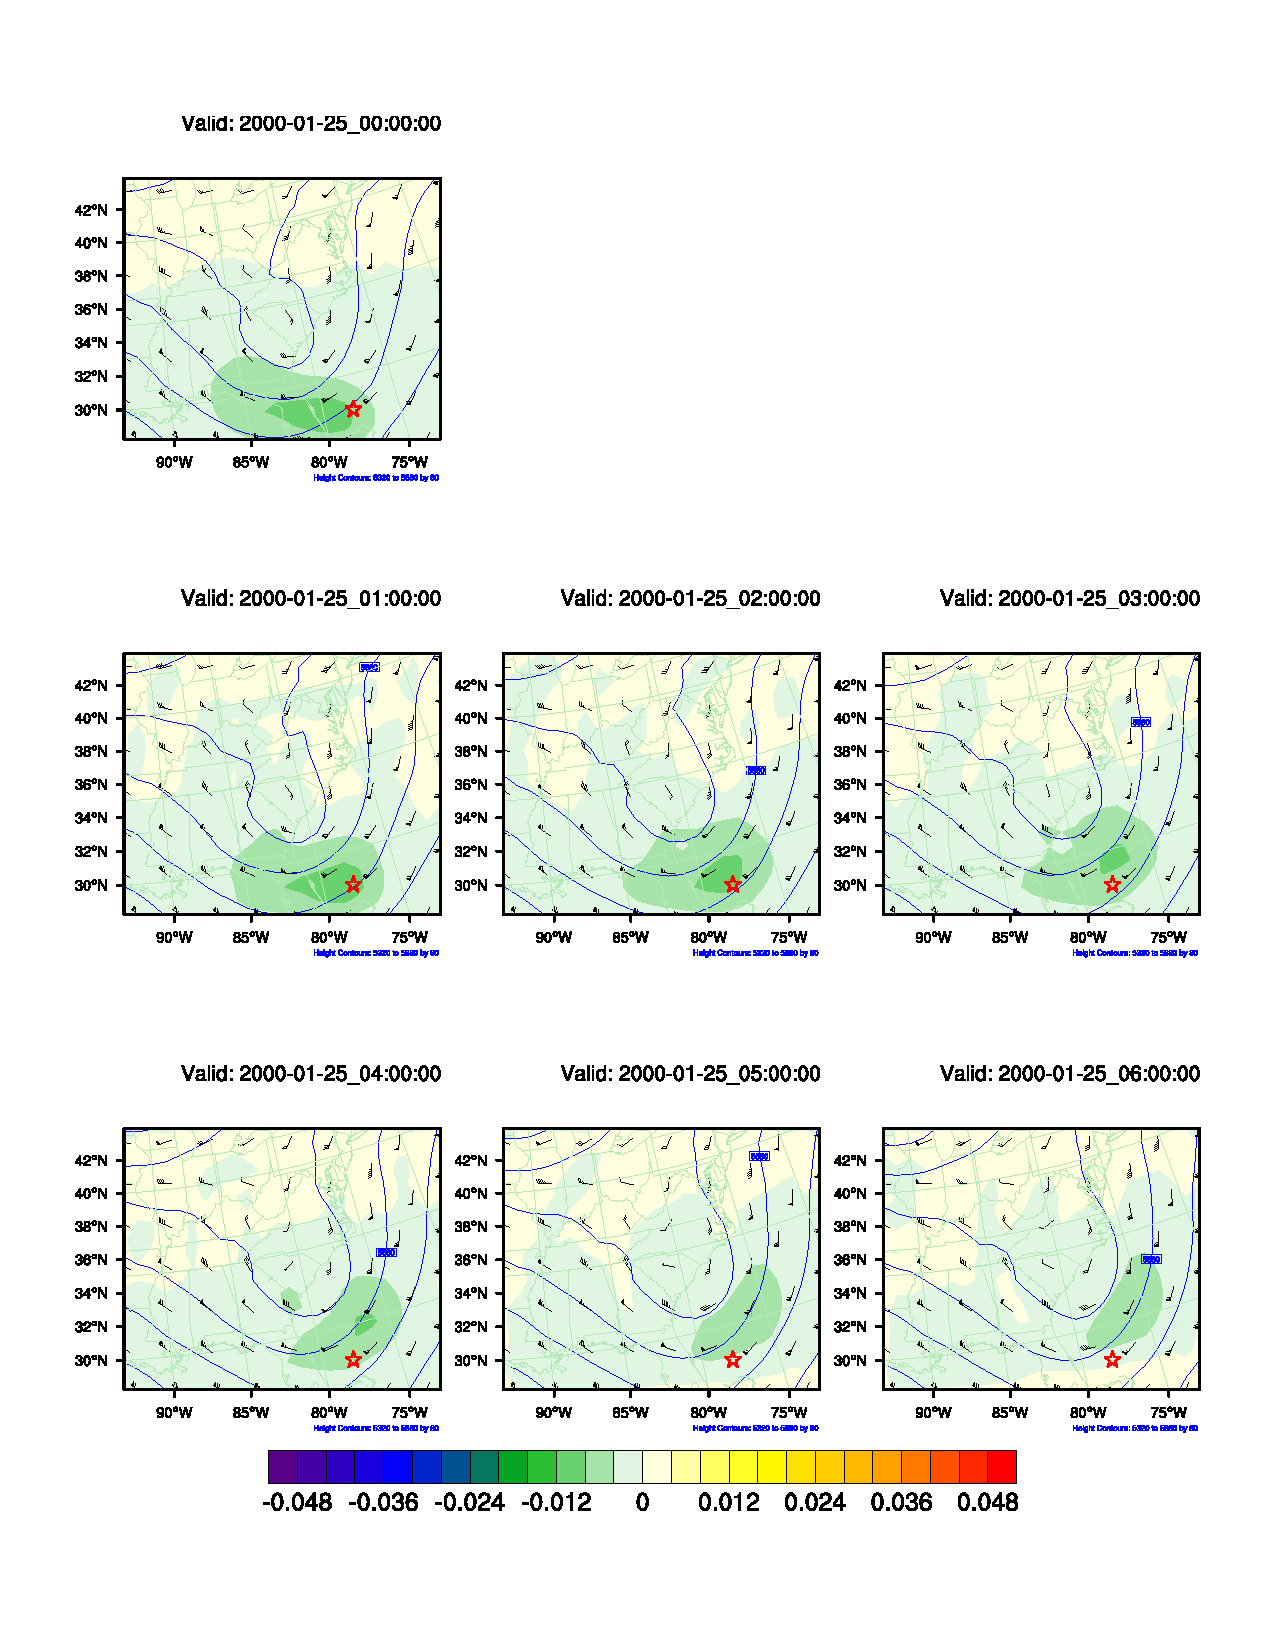
\includegraphics[width=45pc,trim=10 200 10 10, clip, angle=0]{boundarynolbcjcdf.pdf}\\
  \caption{Increment evolution from 0h to 6h. Red star is the obs. location at 6h. LBC control is off.}\label{f3}
\end{figure}
\begin{figure}[t]
  \noindent\includegraphics[width=45pc, trim=10 200 10 10, clip, angle=0]{boundarylbcjcdf.pdf}\\
  \caption{Increment evolution from 0h to 6h. Red star is the obs. location at 6h. LBC control is on.}\label{f4}
\end{figure}
%%%%%%%%%%%%%%%%%%%%%%%%%%%%%%%%%%%%%%%%%%%%%%%%%%%%%%%%%%%%%%%%%%%%%
% TABLES
%%%%%%%%%%%%%%%%%%%%%%%%%%%%%%%%%%%%%%%%%%%%%%%%%%%%%%%%%%%%%%%%%%%%%
%\begin{table}[t]
%\caption{This is a sample table caption and table layout.  Enter as many tables as
 % necessary at the end of your manuscript. Table from Lorenz (1963).}\label{t1}
%\begin{center}
%\begin{tabular}{ccccrrcrc}
%\hline\hline
%$N$ & $X$ & $Y$ & $Z$\\
%\hline
% 0000 & 0000 & 0010 & 0000 \\
% 0005 & 0004 & 0012 & 0000 \\
% 0010 & 0009 & 0020 & 0000 \\
% 0015 & 0016 & 0036 & 0002 \\
% 0020 & 0030 & 0066 & 0007 \\
% 0025 & 0054 & 0115 & 0024 \\
%\hline
%\end{tabular}
%\end{center}
%\end{table}
%
\end{document}